The six archive candidates share Fe\,II 2374 and 2382. This provides a common apparent relative-frequency descriptor, $Y_{\rm app}=-D/c$, where $D=v_{2382}-v_{2374}$. The common redshift cancels, and a shared laboratory-frequency-ratio error contributes a common intercept. The descriptor remains conditional on isotope abundances, gas structure, calibration and the instrumental response. In particular, the much stronger 2382 line is more sensitive to saturation and unresolved structure than 2374. Agreement on ion and lower level does not make the two observed profiles interchangeable.

Before fitting an age trend, we examine the geometry of the six catalogue redshifts alone; no measured shifts enter this calculation. We adopt a flat matter-plus-$\Lambda$ age coordinate with $H_0=67.4\,\mathrm{km\,s^{-1}\,Mpc^{-1}}$, $\Omega_m=0.315$ and no radiation term. These choices define an illustrative age coordinate, not a cosmological fit. The six absorbers span approximately $2.444$--$3.966\,\mathrm{Gyr}$. We fix $t_*=5.391247\times10^{-44}\,\mathrm{s}$ and normalize the proposed family as
\begin{equation}
 G_p(z)=\frac{[\ln(t_0/t_*)/\ln(t(z)/t_*)]^p-1}
 {[\ln(t_0/t_*)/\ln(t(3)/t_*)]^p-1},
 \qquad G_p(0)=0,\quad G_p(3)=1.
 \label{eq:normalized_age}
\end{equation}
In a phenomenological velocity model $D_i=b+A G_2(z_i)$, $A$ is consequently a $z=3$ versus $z=0$ contrast in $\mathrm{m\,s^{-1}}$, extrapolated beyond the candidate redshift range. The sampled $G_2$ span is only $0.262986$: an arbitrary illustrative $A=100\,\mathrm{m\,s^{-1}}$ produces a $26.299\,\mathrm{m\,s^{-1}}$ difference between sample endpoints. This amplitude is neither observed nor predicted by an atomic calculation.

\begin{figure}[htbp]
\centering
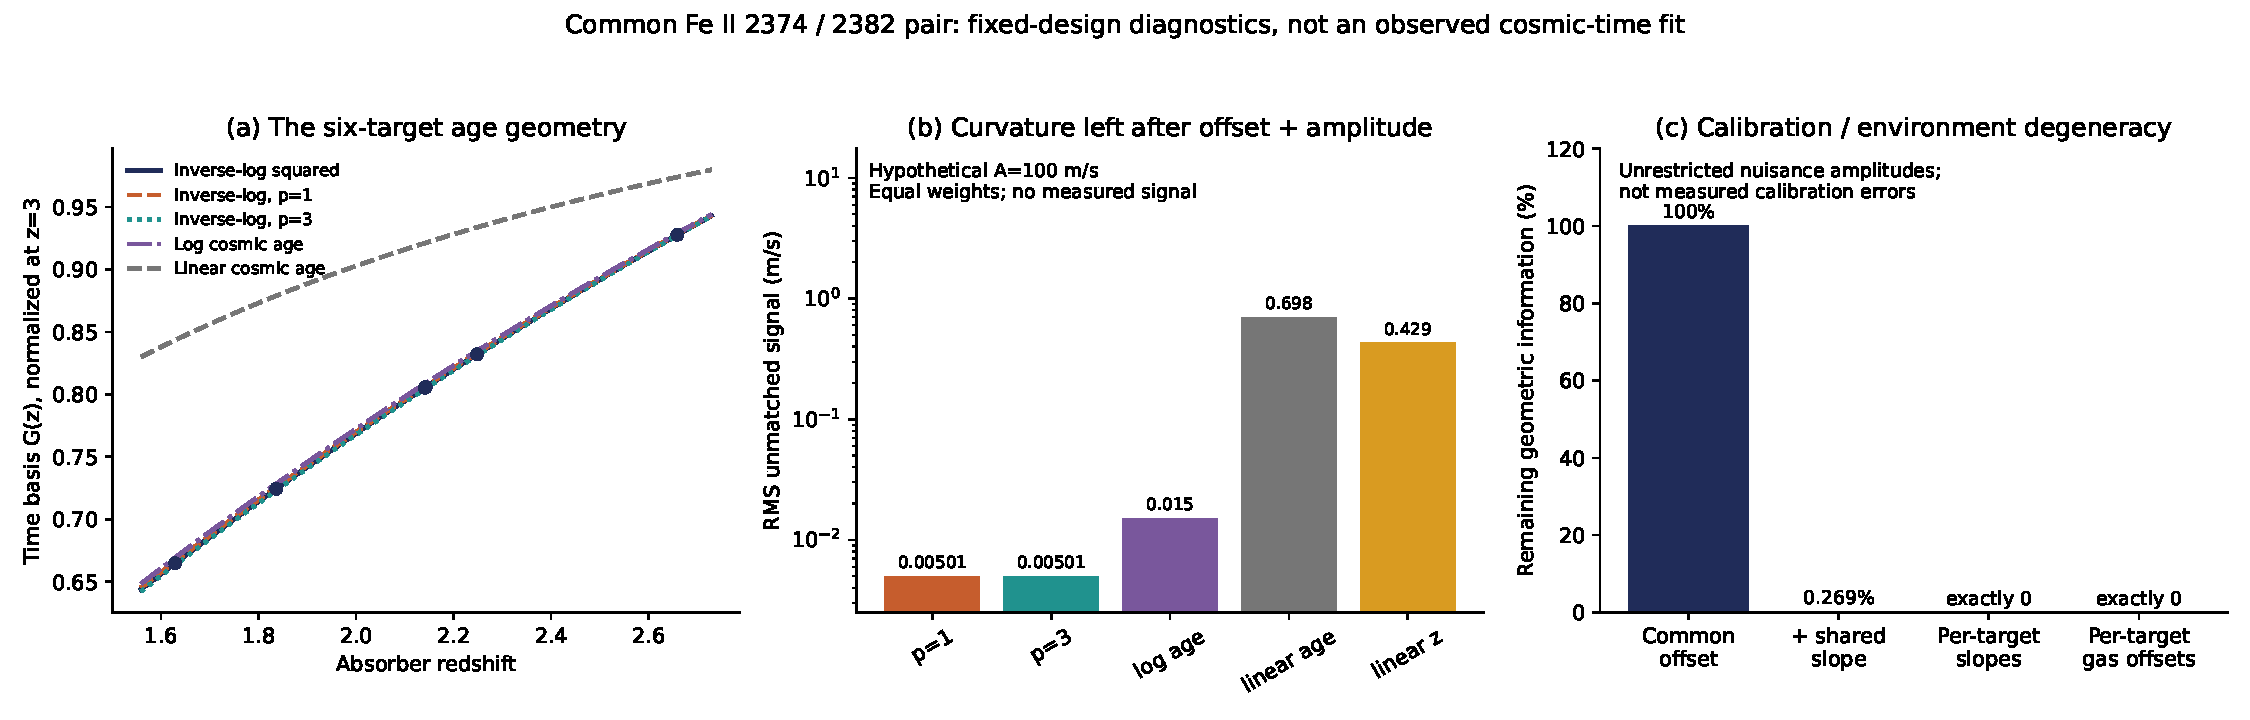
\includegraphics[width=.99\textwidth]{../experiments/highz_feasibility_2026-09-20/results/cross_age/cross_age_identifiability.pdf}
\caption{Fixed-design sensitivity at the six candidate redshifts. The curves and information calculations use no measured line shifts. Free differential offsets for individual absorbers span the age response; more restrictive nuisance assumptions retain conditional information. Competing temporal functions are compared after optimizing their common intercept and amplitude, so raw differences caused only by normalization are removed. All velocity scales in the scenario panels are assumed, not detected.}
\label{fig:age_design}
\end{figure}

The nuisance-space calculation in Fig.~\ref{fig:age_design} illustrates two distinct limitations. Allowing an independently free differential calibration slope for each target gives a full-row-rank nuisance matrix: each slope multiplies a nonzero observed separation of the two transitions. An arbitrary time-amplitude change can then be cancelled exactly. Free target-specific gas or environmental offsets have the same property. This is a statement about identifiability under unrestricted nuisance freedom, not evidence that actual systematics have arbitrary size. A common wavelength zero point cancels between the two lines and cannot produce this degeneracy.

The closeness of this line pair does suppress smooth long-range calibration errors. At the six redshifts its observed separation is approximately $21.83$--$30.38\,\text{\AA}$. Hypothetical velocity-distortion slopes of 50, 200 and $500\,\mathrm{m\,s^{-1}}$ per $1000\,\text{\AA}$ give pair offsets of $1.09$--$1.52$, $4.37$--$6.08$ and $10.92$--$15.19\,\mathrm{m\,s^{-1}}$, respectively. These are propagated scenarios, not adopted empirical priors. If only one slope is shared by all six targets, it leaves $0.269\%$ of the equal-weight age information available with a free intercept alone. However, matching the illustrative $A=100\,\mathrm{m\,s^{-1}}$ age curve actually requires approximately $3077\,\mathrm{m\,s^{-1}}$ per $1000\,\text{\AA}$, with a remaining $0.429\,\mathrm{m\,s^{-1}}$ RMS. Thus a near-degenerate shape cannot be used to claim that modest smooth distortions explain an arbitrarily large effect. Finite independent calibration constraints would restore finite conditional information; short-scale errors and gas-model biases require separate treatment.

Even with those systematics controlled, detecting a trend would not identify its exponent. After re-fitting a common offset and amplitude, $p=1$ and $p=3$ reproduce a $p=2$, $A=100\,\mathrm{m\,s^{-1}}$ scenario to approximately $0.005\,\mathrm{m\,s^{-1}}$ RMS at these six redshifts. An ordinary logarithm of cosmic age differs by $0.015\,\mathrm{m\,s^{-1}}$ RMS, and a linear-age model by $0.698\,\mathrm{m\,s^{-1}}$. These differences arise because a Planck-time reference makes $\ln(t/t_*)$ large compared with its change across this age interval. They scale with the assumed amplitude and are fixed-design model distances, not measured objective differences, detection powers or physical upper bounds.

The pair J053007$-$250329 and J233156$-$090802 is also informative in principle: their rounded catalogue redshifts, 2.141 and 2.143, correspond to an age difference of approximately $2.86\,\mathrm{Myr}$ in this coordinate. The same illustrative age model predicts a difference of only $0.051\,\mathrm{m\,s^{-1}}$. A larger measured difference between such sightlines would test the combined target-dependent effects, provided both descriptors were reliable; it would not uniquely isolate an environmental or instrumental cause. Rounded catalogue redshifts and adopted cosmology do not imply precisely measured ages.

We therefore do not regress the available exploratory offsets into a measured cosmic amplitude. A calibrated cross-age test requires comparable profile constraints, external restrictions on differential systematics, and a specified physical response. The finite set of transitions measures selected energy differences; it does not sample the full symmetry-resolved atomic-level distribution or establish a correspondence to Riemann-zero spacing statistics.
